\PassOptionsToPackage{unicode=true}{hyperref} % options for packages loaded elsewhere
\PassOptionsToPackage{hyphens}{url}
\PassOptionsToPackage{dvipsnames,svgnames*,x11names*}{xcolor}
%
\documentclass[openany]{book}
\usepackage{lmodern}
\usepackage{amssymb,amsmath}
\usepackage{ifxetex,ifluatex}
\usepackage{fixltx2e} % provides \textsubscript
\ifnum 0\ifxetex 1\fi\ifluatex 1\fi=0 % if pdftex
  \usepackage[T1]{fontenc}
  \usepackage[utf8]{inputenc}
  \usepackage{textcomp} % provides euro and other symbols
\else % if luatex or xelatex
  \usepackage{unicode-math}
  \defaultfontfeatures{Ligatures=TeX,Scale=MatchLowercase}
\fi
% use upquote if available, for straight quotes in verbatim environments
\IfFileExists{upquote.sty}{\usepackage{upquote}}{}
% use microtype if available
\IfFileExists{microtype.sty}{%
\usepackage[]{microtype}
\UseMicrotypeSet[protrusion]{basicmath} % disable protrusion for tt fonts
}{}
\IfFileExists{parskip.sty}{%
\usepackage{parskip}
}{% else
\setlength{\parindent}{0pt}
\setlength{\parskip}{6pt plus 2pt minus 1pt}
}
\usepackage{xcolor}
\usepackage{hyperref}
\hypersetup{
            pdftitle={Markdown Exercise},
            pdfauthor={Piet Jonker},
            colorlinks=true,
            linkcolor=Maroon,
            filecolor=Maroon,
            citecolor=Blue,
            urlcolor=red,
            breaklinks=true}
\urlstyle{same}  % don't use monospace font for urls
\usepackage{color}
\usepackage{fancyvrb}
\newcommand{\VerbBar}{|}
\newcommand{\VERB}{\Verb[commandchars=\\\{\}]}
\DefineVerbatimEnvironment{Highlighting}{Verbatim}{commandchars=\\\{\}}
% Add ',fontsize=\small' for more characters per line
\usepackage{framed}
\definecolor{shadecolor}{RGB}{248,248,248}
\newenvironment{Shaded}{\begin{snugshade}}{\end{snugshade}}
\newcommand{\AlertTok}[1]{\textcolor[rgb]{0.94,0.16,0.16}{#1}}
\newcommand{\AnnotationTok}[1]{\textcolor[rgb]{0.56,0.35,0.01}{\textbf{\textit{#1}}}}
\newcommand{\AttributeTok}[1]{\textcolor[rgb]{0.77,0.63,0.00}{#1}}
\newcommand{\BaseNTok}[1]{\textcolor[rgb]{0.00,0.00,0.81}{#1}}
\newcommand{\BuiltInTok}[1]{#1}
\newcommand{\CharTok}[1]{\textcolor[rgb]{0.31,0.60,0.02}{#1}}
\newcommand{\CommentTok}[1]{\textcolor[rgb]{0.56,0.35,0.01}{\textit{#1}}}
\newcommand{\CommentVarTok}[1]{\textcolor[rgb]{0.56,0.35,0.01}{\textbf{\textit{#1}}}}
\newcommand{\ConstantTok}[1]{\textcolor[rgb]{0.00,0.00,0.00}{#1}}
\newcommand{\ControlFlowTok}[1]{\textcolor[rgb]{0.13,0.29,0.53}{\textbf{#1}}}
\newcommand{\DataTypeTok}[1]{\textcolor[rgb]{0.13,0.29,0.53}{#1}}
\newcommand{\DecValTok}[1]{\textcolor[rgb]{0.00,0.00,0.81}{#1}}
\newcommand{\DocumentationTok}[1]{\textcolor[rgb]{0.56,0.35,0.01}{\textbf{\textit{#1}}}}
\newcommand{\ErrorTok}[1]{\textcolor[rgb]{0.64,0.00,0.00}{\textbf{#1}}}
\newcommand{\ExtensionTok}[1]{#1}
\newcommand{\FloatTok}[1]{\textcolor[rgb]{0.00,0.00,0.81}{#1}}
\newcommand{\FunctionTok}[1]{\textcolor[rgb]{0.00,0.00,0.00}{#1}}
\newcommand{\ImportTok}[1]{#1}
\newcommand{\InformationTok}[1]{\textcolor[rgb]{0.56,0.35,0.01}{\textbf{\textit{#1}}}}
\newcommand{\KeywordTok}[1]{\textcolor[rgb]{0.13,0.29,0.53}{\textbf{#1}}}
\newcommand{\NormalTok}[1]{#1}
\newcommand{\OperatorTok}[1]{\textcolor[rgb]{0.81,0.36,0.00}{\textbf{#1}}}
\newcommand{\OtherTok}[1]{\textcolor[rgb]{0.56,0.35,0.01}{#1}}
\newcommand{\PreprocessorTok}[1]{\textcolor[rgb]{0.56,0.35,0.01}{\textit{#1}}}
\newcommand{\RegionMarkerTok}[1]{#1}
\newcommand{\SpecialCharTok}[1]{\textcolor[rgb]{0.00,0.00,0.00}{#1}}
\newcommand{\SpecialStringTok}[1]{\textcolor[rgb]{0.31,0.60,0.02}{#1}}
\newcommand{\StringTok}[1]{\textcolor[rgb]{0.31,0.60,0.02}{#1}}
\newcommand{\VariableTok}[1]{\textcolor[rgb]{0.00,0.00,0.00}{#1}}
\newcommand{\VerbatimStringTok}[1]{\textcolor[rgb]{0.31,0.60,0.02}{#1}}
\newcommand{\WarningTok}[1]{\textcolor[rgb]{0.56,0.35,0.01}{\textbf{\textit{#1}}}}
\usepackage{longtable,booktabs}
% Fix footnotes in tables (requires footnote package)
\IfFileExists{footnote.sty}{\usepackage{footnote}\makesavenoteenv{longtable}}{}
\usepackage{graphicx,grffile}
\makeatletter
\def\maxwidth{\ifdim\Gin@nat@width>\linewidth\linewidth\else\Gin@nat@width\fi}
\def\maxheight{\ifdim\Gin@nat@height>\textheight\textheight\else\Gin@nat@height\fi}
\makeatother
% Scale images if necessary, so that they will not overflow the page
% margins by default, and it is still possible to overwrite the defaults
% using explicit options in \includegraphics[width, height, ...]{}
\setkeys{Gin}{width=\maxwidth,height=\maxheight,keepaspectratio}
\setlength{\emergencystretch}{3em}  % prevent overfull lines
\providecommand{\tightlist}{%
  \setlength{\itemsep}{0pt}\setlength{\parskip}{0pt}}
\setcounter{secnumdepth}{5}
% Redefines (sub)paragraphs to behave more like sections
\ifx\paragraph\undefined\else
\let\oldparagraph\paragraph
\renewcommand{\paragraph}[1]{\oldparagraph{#1}\mbox{}}
\fi
\ifx\subparagraph\undefined\else
\let\oldsubparagraph\subparagraph
\renewcommand{\subparagraph}[1]{\oldsubparagraph{#1}\mbox{}}
\fi

% set default figure placement to htbp
\makeatletter
\def\fps@figure{htbp}
\makeatother

\usepackage{booktabs}
\usepackage{amsmath}
\usepackage{tikz}
\usepackage{pgfplots}
\pgfplotsset{compat=1.17}
\usepackage{amsfonts}
\usepackage{etoolbox}
\makeatletter
\providecommand{\subtitle}[1]{% add subtitle to \maketitle
  \apptocmd{\@title}{\par {\large #1 \par}}{}{}
}
\makeatother
\usepackage[]{natbib}
\bibliographystyle{apalike}

\title{Markdown Exercise}
\providecommand{\subtitle}[1]{}
\subtitle{Using a Random Number Generator to create a cleaning schedule}
\author{Piet Jonker}
\date{2020-10-28}

\begin{document}
\maketitle

{
\hypersetup{linkcolor=}
\setcounter{tocdepth}{1}
\tableofcontents
}
\hypertarget{notes}{%
\chapter*{Notes}\label{notes}}
\addcontentsline{toc}{chapter}{Notes}

\emph{Welcome dear reader}

This document concerns an exercise in writing reproducible code and learning the markdown language in R.

\hypertarget{objectives}{%
\section*{Objectives}\label{objectives}}
\addcontentsline{toc}{section}{Objectives}

Here are some notes on the objectives of this document.

\begin{enumerate}
\def\labelenumi{\arabic{enumi}.}
\tightlist
\item
  The target audience of this document is regarded as the one and only Gerko Vink and possibily classmates
\item
  This document should be reproducible and run flawless on any device
\item
  There should be a glossary, consisting of three parts

  \begin{itemize}
  \tightlist
  \item
    Abbreviations (in text, e.g. \emph{``RNG''})
  \item
    Long form (in glossary, e.g. \emph{``Random Number Generator''})
  \item
    Exhaustive definition (in glossary, e.g. \emph{``A Random Number Generator creates random numbers''})
  \end{itemize}
\item
  Easy to read and use
\item
  Each function will be seperately created and stored in a folder
\item
  Compatability with PDF, and if the glossary allows it also HTML
\end{enumerate}

\hypertarget{gloss}{%
\chapter*{Glossary}\label{gloss}}
\addcontentsline{toc}{chapter}{Glossary}

\begin{description}
\item[\protect\hypertarget{rng}{}{RNG}]
Random Number Generator

Random number generation (RNG) is a process which, through a device, generates a sequence of numbers or symbols that cannot be reasonably predicted better than by a random chance. Random number generators can be true hardware random-number generators (HRNGS), which generate random numbers as a function of current value of some physical environment attribute that is constantly changing in a manner that is practically impossible to model, or pseudo-random number generators (PRNGS), which generate numbers that look random, but are actually deterministic, and can be reproduced if the state of the PRNG is known.
\end{description}

\hypertarget{intro}{%
\chapter{Introduction}\label{intro}}

\hypertarget{background}{%
\section{Background}\label{background}}

Students at both selective and nonselective institutions frequently engage in academic procrastination regardless of their gender, race, or learning style. Studies indicate that fear of failure, aversiveness of the task, and fear of social disapproval by peers are primary motives for academic procrastination. \cite{einstein} found that academic and non-academic tasks should be challenging, yet fun, to heighten the likelihood that they are completed by students.

This document will aim to challenge the author in a fun way, as suggested by \cite{einstein}. Three methods of which two use a \protect\hyperlink{rng}{RNG} will be deployed to automatically create a cleaning schedule for a six person household with three cleaning tasks. This creates a challenge that is fun and a solution to a relevant problem which the author faces.

Since we've established that procrastination is bad, we can postulate that it is desirable to minimize the amount of effort that needs to be undertaken in order to fulfill tasks, such as household chores. In student housing, cleaning schedules are often used as tool to plan divide tasks. However, student housing is a high throughput system where residents often move to other places and new roommates take their place. This immediatly causes the schedule to be outdated. Furthermore, the schedule can be outdated. Both factors cause the schedule to be outdated as we can see in Figure 1.

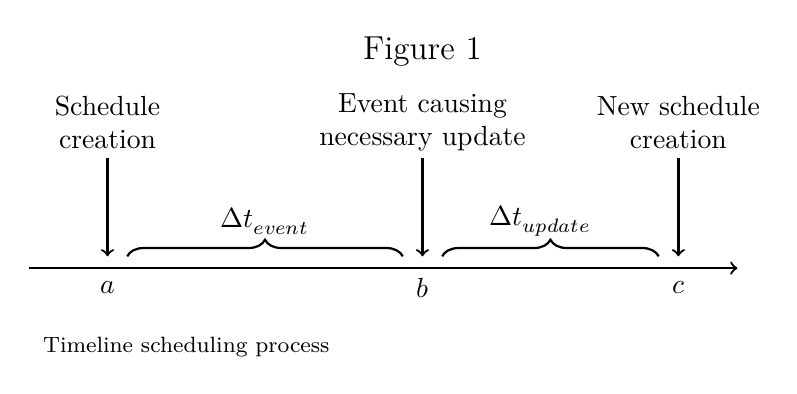
\begin{tikzpicture}[scale=1]

  % title
  \node [align=center] at (5,    2.75)   {\large Figure 1};
  
  % subtitle
  \node [align=center] at (2,    -1)     {\footnotesize \text{Timeline scheduling process}};
  
  % time points
  \node [align=center] at (1,    1.85)   {Schedule\\creation};
  \node [align=center] at (5,    1.85)   {Event causing\\necessary update};
  \node [align=center] at (8.25, 1.85)   {New schedule\\creation};
  
  % mathematical notation of time points
  \node [align=center] at (1,    -0.25)  {$a$};
  \node [align=center] at (5,    -0.25)  {$b$};
  \node [align=center] at (8.25, -0.25)  {$c$};
  
  % mathematical notation of time spans
  \node [align=center] at (3,      0.6)    {$\Delta t_{event}$};
  \node [align=center] at (6.5,    0.6)    {$\Delta t_{update}$};
  
  % arrows 
  \draw [thick,->]        (1,    1.4) -- (1,    0.15);
  \draw [thick,->]        (5,    1.4) -- (5,    0.15);
  \draw [thick,->]        (8.25, 1.4) -- (8.25, 0.15);  
  \draw [thick,->]        (0,    0)   -- (9,    0);
  
  % braces
  \draw [thick,decorate,decoration={brace,amplitude=6pt,raise=0pt}] 
                          (1.25, 0.15) -- (4.75, 0.15);
  \draw [thick,decorate,decoration={brace,amplitude=6pt,raise=0pt}] 
                          (5.25, 0.15) -- (8,    0.15);
                          
\end{tikzpicture}

A new schedule will take effort to make, causing an increase of \(\Delta t_{update}\). To minimalize \(\Delta t_{update}\), it is useful to automate process \(b\) as much as possible. In order to achieve this goal an approach to automate this process will be presented. This way we follow the guidelines by \cite{einstein} in the sense that it makes this assignment challenging, fun, but also useful.

It should have the following structure:

\begin{longtable}[]{@{}llll@{}}
\toprule
Date & Chore 1 & Chore 2 & Chore 3\tabularnewline
\midrule
\endhead
Date 1 & Name roommate & Name roommate & Name roommate\tabularnewline
Date 2 & Name roommate & Name roommate & Name roommate\tabularnewline
\bottomrule
\end{longtable}

\hypertarget{method}{%
\chapter{Method}\label{method}}

\hypertarget{deterministic-versus-random-number-generator}{%
\section{Deterministic versus Random Number Generator}\label{deterministic-versus-random-number-generator}}

The Random Number Generator will be used to divide tasks among roommates in a pseudo-random manner. This will then be compared to a deterministic approach so that the two methods can be compared.

First the seed is set so that our results are reproducible. Also, the tidyverse is loaded since we'll need it later.

\begin{Shaded}
\begin{Highlighting}[]
\KeywordTok{library}\NormalTok{(tidyverse)}
\KeywordTok{library}\NormalTok{(knitr)}
\KeywordTok{set.seed}\NormalTok{(}\DecValTok{123}\NormalTok{)}
\end{Highlighting}
\end{Shaded}

\hypertarget{deterministic-approach}{%
\subsection*{Deterministic approach}\label{deterministic-approach}}
\addcontentsline{toc}{subsection}{Deterministic approach}

First a function will be created for the deterministic approach. One pattern will repeat itself for the entire sequence of dates specified. We will do this as following:

\begin{Shaded}
\begin{Highlighting}[]
\NormalTok{createSchedule <-}\StringTok{ }\ControlFlowTok{function}\NormalTok{(}\DataTypeTok{startDate =} \KeywordTok{Sys.Date}\NormalTok{(),         }\CommentTok{# the current date is used as default input}
                           \DataTypeTok{endDate   =} \KeywordTok{Sys.Date}\NormalTok{() }\OperatorTok{+}\StringTok{ }\DecValTok{305}\NormalTok{,   }\CommentTok{# }
                           \DataTypeTok{createCSV =} \StringTok{"no"}\NormalTok{,                           }
\NormalTok{                           roommateNames}
\NormalTok{                           ) \{}

  \CommentTok{# create a string of dates between startDate and endDate}
\NormalTok{  dateString <-}\StringTok{ }\KeywordTok{seq}\NormalTok{(}\DataTypeTok{from =}\NormalTok{ startDate,}
                    \DataTypeTok{to   =}\NormalTok{ endDate,}
                    \DataTypeTok{by   =} \StringTok{"days"}\NormalTok{)}

  \CommentTok{# turn it into dataframe}
\NormalTok{  data <-}\StringTok{ }\KeywordTok{as.data.frame}\NormalTok{(dateString)}

  \CommentTok{# add weekdays}
\NormalTok{  data <-}\StringTok{ }\NormalTok{data }\OperatorTok
\StringTok{    }\KeywordTok{mutate}\NormalTok{(}\DataTypeTok{days =} \KeywordTok{weekdays}\NormalTok{(dateString))}

  \CommentTok{# filter out fridays}
\NormalTok{  data <-}\StringTok{ }\NormalTok{data }\OperatorTok
\StringTok{    }\KeywordTok{filter}\NormalTok{(days }\OperatorTok{==}\StringTok{ "vrijdag"} \OperatorTok{|}\StringTok{ }\NormalTok{days }\OperatorTok{==}\StringTok{ "friday"}\NormalTok{)}

  \CommentTok{# shuffle the orders of the name strings so that they can be put into dataframe}
\NormalTok{  roommateNames2 <-}\StringTok{ }\NormalTok{roommateNames[}\KeywordTok{c}\NormalTok{(}\DecValTok{5}\NormalTok{,}\DecValTok{6}\NormalTok{,}\DecValTok{1}\NormalTok{,}\DecValTok{2}\NormalTok{,}\DecValTok{3}\NormalTok{,}\DecValTok{4}\NormalTok{)]}
\NormalTok{  roommateNames3 <-}\StringTok{ }\NormalTok{roommateNames[}\KeywordTok{c}\NormalTok{(}\DecValTok{3}\NormalTok{,}\DecValTok{4}\NormalTok{,}\DecValTok{5}\NormalTok{,}\DecValTok{6}\NormalTok{,}\DecValTok{1}\NormalTok{,}\DecValTok{2}\NormalTok{)]}

  \CommentTok{# add columns with chores}
\NormalTok{  data <-}\StringTok{ }\NormalTok{data }\OperatorTok
\StringTok{    }\KeywordTok{mutate}\NormalTok{(}\DataTypeTok{gang     =} \KeywordTok{rep_len}\NormalTok{(roommateNames,  }\DataTypeTok{length.out =} \KeywordTok{nrow}\NormalTok{(data)),}
           \DataTypeTok{keuken   =} \KeywordTok{rep_len}\NormalTok{(roommateNames2, }\DataTypeTok{length.out =} \KeywordTok{nrow}\NormalTok{(data)),}
           \DataTypeTok{badkamer =} \KeywordTok{rep_len}\NormalTok{(roommateNames3, }\DataTypeTok{length.out =} \KeywordTok{nrow}\NormalTok{(data))}
\NormalTok{           )}

  \CommentTok{# format dates}
\NormalTok{  data <-}\StringTok{ }\NormalTok{data }\OperatorTok
\StringTok{    }\KeywordTok{mutate}\NormalTok{(}\DataTypeTok{datum =} \KeywordTok{format}\NormalTok{(dateString, }\StringTok{"%d-%m-%y"}\NormalTok{))}

  \CommentTok{# delete weekday and dateString column}
\NormalTok{  data <-}\StringTok{ }\NormalTok{data }\OperatorTok
\StringTok{    }\KeywordTok{select}\NormalTok{(datum, }
\NormalTok{           gang,}
\NormalTok{           keuken, }
\NormalTok{           badkamer)}
  
  \ControlFlowTok{if}\NormalTok{ (createCSV }\OperatorTok{==}\StringTok{ "yes"}\NormalTok{) \{}
    \KeywordTok{write.csv}\NormalTok{(data, }\DataTypeTok{file =} \StringTok{"schedule.csv"}\NormalTok{)}
\NormalTok{  \} }\ControlFlowTok{else}\NormalTok{ \{}
      \KeywordTok{return}\NormalTok{(data)}
\NormalTok{  \}}
  
\NormalTok{\}}
\end{Highlighting}
\end{Shaded}

Now, we test the function and show the first 10 rows of the schedule. To do this in a reproducible manner, we specify:

\begin{itemize}
\tightlist
\item
  a start date
\item
  an end date
\item
  the names of my roommates
\end{itemize}

This will be used throughout this document. Completely by chance, the start date is my birthday and the end date Sinterklaas evening (which is my grandfathers birthday).

\begin{Shaded}
\begin{Highlighting}[]
\NormalTok{startDate     <-}\StringTok{ }\KeywordTok{as.Date}\NormalTok{(}\StringTok{"1996-02-16"}\NormalTok{)}
\NormalTok{endDate       <-}\StringTok{ }\KeywordTok{as.Date}\NormalTok{(}\StringTok{"1996-12-15"}\NormalTok{) }
\NormalTok{roommateNames <-}\StringTok{ }\KeywordTok{c}\NormalTok{(}\StringTok{"thijs"}\NormalTok{, }\StringTok{"jur"}\NormalTok{, }\StringTok{"wies"}\NormalTok{, }\StringTok{"hidde"}\NormalTok{, }\StringTok{"piet"}\NormalTok{, }\StringTok{"jette"}\NormalTok{)}

\KeywordTok{kable}\NormalTok{(}\KeywordTok{createSchedule}\NormalTok{(}\DataTypeTok{startDate     =}\NormalTok{ startDate,}
                     \DataTypeTok{endDate       =}\NormalTok{ endDate,}
                     \DataTypeTok{createCSV     =} \StringTok{"no"}\NormalTok{, }
                     \DataTypeTok{roommateNames =}\NormalTok{ roommateNames)[}\DecValTok{1}\OperatorTok{:}\DecValTok{10}\NormalTok{,])}
\end{Highlighting}
\end{Shaded}

\begin{tabular}{l|l|l|l}
\hline
datum & gang & keuken & badkamer\\
\hline
16-02-96 & thijs & piet & wies\\
\hline
23-02-96 & jur & jette & hidde\\
\hline
01-03-96 & wies & thijs & piet\\
\hline
08-03-96 & hidde & jur & jette\\
\hline
15-03-96 & piet & wies & thijs\\
\hline
22-03-96 & jette & hidde & jur\\
\hline
29-03-96 & thijs & piet & wies\\
\hline
05-04-96 & jur & jette & hidde\\
\hline
12-04-96 & wies & thijs & piet\\
\hline
19-04-96 & hidde & jur & jette\\
\hline
\end{tabular}

\hypertarget{rng-approach-1}{%
\subsection*{RNG approach 1}\label{rng-approach-1}}
\addcontentsline{toc}{subsection}{RNG approach 1}

In this version, we use the sample function to sample one name per chore per week, The sample function uses the \protect\hyperlink{rng}{RNG}. This approach might not be the most convenient, since it is possible for one person to have all the chores in a given week.

\begin{Shaded}
\begin{Highlighting}[]
\NormalTok{createScheduleFull <-}\StringTok{ }\ControlFlowTok{function}\NormalTok{(}\DataTypeTok{startDate =} \KeywordTok{Sys.Date}\NormalTok{(),}
                               \DataTypeTok{endDate   =} \KeywordTok{Sys.Date}\NormalTok{() }\OperatorTok{+}\StringTok{ }\DecValTok{305}\NormalTok{,}
                               \DataTypeTok{createCSV =} \StringTok{"no"}\NormalTok{,                           }
\NormalTok{                               roommateNames}
\NormalTok{                           ) \{}

  \CommentTok{# create a string of dates between startDate and endDate}
\NormalTok{  dateString <-}\StringTok{ }\KeywordTok{seq}\NormalTok{(}\DataTypeTok{from =}\NormalTok{ startDate,}
                    \DataTypeTok{to   =}\NormalTok{ endDate,}
                    \DataTypeTok{by   =} \StringTok{"days"}\NormalTok{)}

  \CommentTok{# turn it into dataframe}
\NormalTok{  data <-}\StringTok{ }\KeywordTok{as.data.frame}\NormalTok{(dateString)}

  \CommentTok{# add weekdays}
\NormalTok{  data <-}\StringTok{ }\NormalTok{data }\OperatorTok
\StringTok{    }\KeywordTok{mutate}\NormalTok{(}\DataTypeTok{days =} \KeywordTok{weekdays}\NormalTok{(dateString))}

  \CommentTok{# filter out fridays}
\NormalTok{  data <-}\StringTok{ }\NormalTok{data }\OperatorTok
\StringTok{    }\KeywordTok{filter}\NormalTok{(days }\OperatorTok{==}\StringTok{ "vrijdag"} \OperatorTok{|}\StringTok{ }\NormalTok{days }\OperatorTok{==}\StringTok{ "friday"}\NormalTok{)}
  
\NormalTok{  data <-}\StringTok{ }\NormalTok{data }\OperatorTok\StringTok{ }
\StringTok{    }\KeywordTok{rowwise}\NormalTok{() }\OperatorTok\StringTok{ }
\StringTok{    }\KeywordTok{mutate}\NormalTok{(}\DataTypeTok{gang     =} \KeywordTok{sample}\NormalTok{(roommateNames, }\DecValTok{1}\NormalTok{, }\DataTypeTok{replace =} \OtherTok{TRUE}\NormalTok{),}
           \DataTypeTok{keuken   =} \KeywordTok{sample}\NormalTok{(roommateNames, }\DecValTok{1}\NormalTok{, }\DataTypeTok{replace =} \OtherTok{TRUE}\NormalTok{),}
           \DataTypeTok{badkamer =} \KeywordTok{sample}\NormalTok{(roommateNames, }\DecValTok{1}\NormalTok{, }\DataTypeTok{replace =} \OtherTok{TRUE}\NormalTok{)}
\NormalTok{           )}
  
  \CommentTok{# format dates}
\NormalTok{  data <-}\StringTok{ }\NormalTok{data }\OperatorTok
\StringTok{    }\KeywordTok{mutate}\NormalTok{(}\DataTypeTok{datum =} \KeywordTok{format}\NormalTok{(dateString, }\StringTok{"%d-%m-%y"}\NormalTok{))}

  \CommentTok{# delete weekday column and rename}
\NormalTok{  data <-}\StringTok{ }\NormalTok{data }\OperatorTok
\StringTok{    }\KeywordTok{select}\NormalTok{(datum, }
\NormalTok{           gang,}
\NormalTok{           keuken, }
\NormalTok{           badkamer)}
  
  \ControlFlowTok{if}\NormalTok{ (createCSV }\OperatorTok{==}\StringTok{ "yes"}\NormalTok{) \{}
    \KeywordTok{write.csv}\NormalTok{(data, }\DataTypeTok{file =} \StringTok{"schedule.csv"}\NormalTok{)}
\NormalTok{  \} }\ControlFlowTok{else}\NormalTok{ \{}
      \KeywordTok{return}\NormalTok{(data)}
\NormalTok{  \}}
  
\NormalTok{\}}
\end{Highlighting}
\end{Shaded}

Again, we test the function and show the first 10 rows

\begin{Shaded}
\begin{Highlighting}[]
\KeywordTok{kable}\NormalTok{(}\KeywordTok{createScheduleFull}\NormalTok{(}\DataTypeTok{startDate     =}\NormalTok{ startDate,}
                     \DataTypeTok{endDate       =}\NormalTok{ endDate,}
                     \DataTypeTok{createCSV     =} \StringTok{"no"}\NormalTok{, }
                     \DataTypeTok{roommateNames =}\NormalTok{ roommateNames)[}\DecValTok{1}\OperatorTok{:}\DecValTok{10}\NormalTok{,])}
\end{Highlighting}
\end{Shaded}

\begin{tabular}{l|l|l|l}
\hline
datum & gang & keuken & badkamer\\
\hline
16-02-96 & wies & jette & jette\\
\hline
23-02-96 & jette & thijs & wies\\
\hline
01-03-96 & wies & jur & jette\\
\hline
08-03-96 & jur & piet & piet\\
\hline
15-03-96 & jur & piet & wies\\
\hline
22-03-96 & jette & hidde & jette\\
\hline
29-03-96 & wies & piet & jur\\
\hline
05-04-96 & piet & jur & piet\\
\hline
12-04-96 & hidde & thijs & piet\\
\hline
19-04-96 & jette & thijs & wies\\
\hline
\end{tabular}

\hypertarget{rng-approach-2}{%
\subsection*{RNG approach 2}\label{rng-approach-2}}
\addcontentsline{toc}{subsection}{RNG approach 2}

Now, we create the another function which uses the sample function to pick roommates for chores. Every other week three names from the string of six names will be randomly assigned for a task. The next week, the three remaining names from that sample will be assigned. This way, a random sample is taken, but we avoid the problem of someone having multiple chores in one week.

\begin{Shaded}
\begin{Highlighting}[]
\NormalTok{createScheduleSemi <-}\StringTok{ }\ControlFlowTok{function}\NormalTok{(}\DataTypeTok{startDate =} \KeywordTok{Sys.Date}\NormalTok{(),}
                           \DataTypeTok{endDate   =} \KeywordTok{Sys.Date}\NormalTok{() }\OperatorTok{+}\StringTok{ }\DecValTok{305}\NormalTok{,}
                           \DataTypeTok{createCSV =} \StringTok{"no"}\NormalTok{,                           }
\NormalTok{                           roommateNames}
\NormalTok{                           ) \{}

  \CommentTok{# create a string of dates between startDate and endDate}
\NormalTok{  dateString <-}\StringTok{ }\KeywordTok{seq}\NormalTok{(}\DataTypeTok{from =}\NormalTok{ startDate,}
                    \DataTypeTok{to   =}\NormalTok{ endDate,}
                    \DataTypeTok{by   =} \StringTok{"days"}\NormalTok{)}

  \CommentTok{# turn it into dataframe}
\NormalTok{  data <-}\StringTok{ }\KeywordTok{as.data.frame}\NormalTok{(dateString)}

  \CommentTok{# add weekdays}
\NormalTok{  data <-}\StringTok{ }\NormalTok{data }\OperatorTok
\StringTok{    }\KeywordTok{mutate}\NormalTok{(}\DataTypeTok{days =} \KeywordTok{weekdays}\NormalTok{(dateString))}

  \CommentTok{# filter out fridays}
\NormalTok{  data <-}\StringTok{ }\NormalTok{data }\OperatorTok
\StringTok{    }\KeywordTok{filter}\NormalTok{(days }\OperatorTok{==}\StringTok{ "vrijdag"} \OperatorTok{|}\StringTok{ }\NormalTok{days }\OperatorTok{==}\StringTok{ "friday"}\NormalTok{)}

  \CommentTok{# draw a random sample, fill the first row with the first three elements of the sampled vector and the row after with the remaining three elements of the sampled vector}
 \ControlFlowTok{for}\NormalTok{(i }\ControlFlowTok{in} \KeywordTok{seq}\NormalTok{(}\DataTypeTok{from =} \DecValTok{1}\NormalTok{, }\DataTypeTok{to =} \KeywordTok{nrow}\NormalTok{(data), }\DataTypeTok{by =} \DecValTok{2}\NormalTok{))\{}
\NormalTok{    sample       <-}\StringTok{ }\KeywordTok{sample}\NormalTok{(roommateNames, }\DecValTok{6}\NormalTok{)}
\NormalTok{    data[i,}\DecValTok{3}\NormalTok{]    <-}\StringTok{ }\NormalTok{sample[}\DecValTok{1}\NormalTok{]}
\NormalTok{    data[i,}\DecValTok{4}\NormalTok{]    <-}\StringTok{ }\NormalTok{sample[}\DecValTok{2}\NormalTok{]}
\NormalTok{    data[i,}\DecValTok{5}\NormalTok{]    <-}\StringTok{ }\NormalTok{sample[}\DecValTok{3}\NormalTok{]}
\NormalTok{    data[i}\OperatorTok{+}\DecValTok{1}\NormalTok{, }\DecValTok{3}\NormalTok{] <-}\StringTok{ }\NormalTok{sample[}\DecValTok{4}\NormalTok{]}
\NormalTok{    data[i}\OperatorTok{+}\DecValTok{1}\NormalTok{, }\DecValTok{4}\NormalTok{] <-}\StringTok{ }\NormalTok{sample[}\DecValTok{5}\NormalTok{]}
\NormalTok{    data[i}\OperatorTok{+}\DecValTok{1}\NormalTok{, }\DecValTok{5}\NormalTok{] <-}\StringTok{ }\NormalTok{sample[}\DecValTok{6}\NormalTok{]}
\NormalTok{ \}}
  
  \CommentTok{# rename columns for clarity}
\NormalTok{ data <-}\StringTok{ }\NormalTok{data }\OperatorTok\StringTok{ }
\StringTok{   }\KeywordTok{rename}\NormalTok{(}\DataTypeTok{gang     =}\NormalTok{ V3,}
          \DataTypeTok{keuken   =}\NormalTok{ V4,}
          \DataTypeTok{badkamer =}\NormalTok{ V5)}
 
  \CommentTok{# format dates}
\NormalTok{  data <-}\StringTok{ }\NormalTok{data }\OperatorTok
\StringTok{    }\KeywordTok{mutate}\NormalTok{(}\DataTypeTok{datum =} \KeywordTok{format}\NormalTok{(dateString, }\StringTok{"%d-%m-%y"}\NormalTok{))}

  \CommentTok{# delete weekday column and rename}
\NormalTok{  data <-}\StringTok{ }\NormalTok{data }\OperatorTok
\StringTok{    }\KeywordTok{select}\NormalTok{(datum, }
\NormalTok{           gang,}
\NormalTok{           keuken, }
\NormalTok{           badkamer)}
  
  \ControlFlowTok{if}\NormalTok{ (createCSV }\OperatorTok{==}\StringTok{ "yes"}\NormalTok{) \{}
    \KeywordTok{write.csv}\NormalTok{(data, }\DataTypeTok{file =} \StringTok{"schedule.csv"}\NormalTok{)}
\NormalTok{  \} }\ControlFlowTok{else}\NormalTok{ \{}
      \KeywordTok{return}\NormalTok{(data)}
\NormalTok{  \}}
  
\NormalTok{\}}
\end{Highlighting}
\end{Shaded}

Again, we test the function and show the first 10 rows

\begin{Shaded}
\begin{Highlighting}[]
\KeywordTok{kable}\NormalTok{(}\KeywordTok{createScheduleSemi}\NormalTok{(}\DataTypeTok{startDate     =}\NormalTok{ startDate,}
                         \DataTypeTok{endDate       =}\NormalTok{ endDate,}
                         \DataTypeTok{createCSV     =} \StringTok{"no"}\NormalTok{, }
                         \DataTypeTok{roommateNames =}\NormalTok{ roommateNames)[}\DecValTok{1}\OperatorTok{:}\DecValTok{10}\NormalTok{,])}
\end{Highlighting}
\end{Shaded}

\begin{tabular}{l|l|l|l}
\hline
datum & gang & keuken & badkamer\\
\hline
16-02-96 & piet & wies & thijs\\
\hline
23-02-96 & jette & jur & hidde\\
\hline
01-03-96 & thijs & jur & hidde\\
\hline
08-03-96 & jette & wies & piet\\
\hline
15-03-96 & hidde & jette & thijs\\
\hline
22-03-96 & jur & wies & piet\\
\hline
29-03-96 & thijs & wies & hidde\\
\hline
05-04-96 & piet & jette & jur\\
\hline
12-04-96 & hidde & jette & jur\\
\hline
19-04-96 & thijs & piet & wies\\
\hline
\end{tabular}

We have now showed three methods to create schedules, where two use a RNG. I would really like to do an analysis go into depth on the statistics of the approaches such as double or triple assignments in a week. Also, I could have done some form of simulation to see if the approaches are fair when done X amount of times.

Unfortunetaly, most of my time went into creating the bookdown/markdown format, so I'll save this part for a later endeavour. Thanks for reading!

\bibliography{book.bib}

\end{document}
